\section{Proposed Neural Networks}
\label{sec:proposed_networks}

For all networks, varing backbones used to encode state information from observations for both actor and critic networks. 
In critic network, actions are concatenated by state information coming from backbones. 
Then, this concatenated vector is passed through feed forward layer with GELU activation then a linear layer with single output. 
Before feeding observations to backbone, they are passed through a layer with layer normalization with tanh activation to 96 dimensional output. 
In actor network, backbone is followed by a single layer with tanh activation for action estimation. 
As backbones, following networks are proposed. 
Again, observations are passed through a layer with layer normalization with tanh activation to 96 dimensional output before feeding to backbone. 
Critic and Actor networks are illustrated in \figref{fig:nets} 

\begin{figure}
	\begin{subfigure}{.5\textwidth}
		\centering
		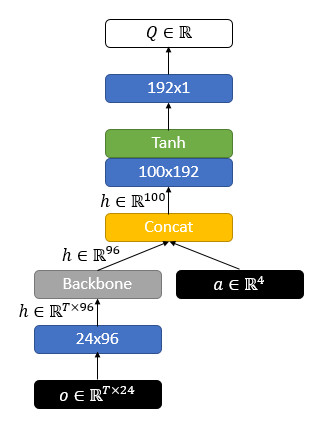
\includegraphics[width=0.97\linewidth]{figures/nets/critic.png}
		\caption{Critic Architecture}
		\label{fig:critic_net}
	\end{subfigure}
	\begin{subfigure}{.5\textwidth}
		\centering
		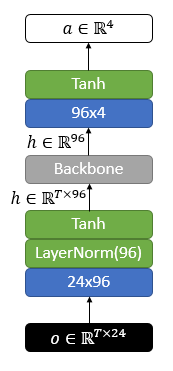
\includegraphics[width=0.55\linewidth]{figures/nets/actor.png}
		\caption{Actor Architecture}
		\label{fig:actor_net}
	\end{subfigure}
	\caption{Neural Architecture Design}
	\label{fig:nets}
\end{figure}

\subsection{Residual Feed Forward Network}

Incoming vector is passed through 2 layers with 192 dimensional hidden size and 96 dimensional output, where there is GELU activation between 2 layers. 
This output is summed with initial vector and this is lastly passed through layer normalization. 

\subsection{Long Short Term Memory}

Sequence of incoming vectors is passed though single layer vanilla LSTM layer with 96 dimensional hidden state. 
Output at last time step is outputted. 

\subsection{Transformer (Pre-layer Normalized)}

Sequence of incoming vectors is passed through single layer pre-layer normalized transformer with 192 dimensional feed forward layer with GELU activation. 
The output is lastly passed through layer normalization. 
During multi-head attention, only the last state is fed as query so that attentions are calculated for only last state. 

